\documentclass[journal]{IEEEtran}
\usepackage[a5paper,margin=10mm]{geometry}
\usepackage{tfrupee}
\setlength{\headheight}{1cm}
\setlength{\headsep}{0mm}
\usepackage{graphicx}
\usepackage{gvv-book}
\usepackage{gvv}
\usetikzlibrary{patterns}
\lstset{aboveskip=12pt}
\usepackage[center]{caption}
\raggedbottom
\hypersetup{colorlinks=true,urlcolor=black,linkcolor=black,citecolor=black,hypertexnames=false,pdftitle={CBSE Mathematics 2015 - Class X, Code 30/1}}
\usepackage{amsfonts}
\makeindex

\begin{document}
\bibliographystyle{IEEEtran}
\onecolumn

\title{
  \begin{center}
    CBSE Mathematics 2015\\
    \rule{0.4\columnwidth}{0.4pt}\\
    Class X -- Outside Delhi, Code 30/1
  \end{center}
}
\author{
  \vspace{2cm}
  \begin{center}
    
\includegraphics[width=0.18\columnwidth]{figs/logo}\\[4pt]
    {\large Formula-first worked solutions with matrix methods}
  \end{center}
}
\maketitle
\newpage

\section*{Scope and source audit}
This build intentionally covers only the Class X Mathematics paper with code 30/1.
The official CBSE paper has 31 questions: Section A (Q1--4), Section B (Q5--10),
Section C (Q11--20), and Section D (Q21--31). Class XII is left out of this build
until the Class X layout and verification pass are finalized.

The solutions state the general formulae first and refer back to them when solving
individual questions. Coordinate-geometry work is expressed with vectors, dot
products, determinants, and matrix systems wherever that makes the reasoning clearer.
The level of mathematics is deliberately enriched, but each solution still gives a
short path to the requested school-level result. Comments in the source files explain
why a particular method is selected; they are mathematical teaching notes rather than
an unfiltered private reasoning trace.

Primary source: official CBSE 2015 paper 30/1 and the corresponding marking scheme.
The source audit records transcription mismatches in \texttt{STRUCTURE\_AUDIT.md}.

\newpage
\tableofcontents
\newpage
\numberwithin{equation}{enumi}
\numberwithin{figure}{enumi}
\renewcommand{\thetable}{\theenumi}

\section{Class X Mathematics -- Code 30/1}
\subsection{Formulae}
% Formula sheet comes before every worked question.  Equation tags F1, F2, ...
% keep this reference sheet distinguishable from equations numbered by question.
\renewcommand{\theequation}{F\arabic{equation}}
\setcounter{equation}{0}

\subsubsection*{1. Quadratic equations and algebra}
For $ax^2+bx+c=0$ with $a\ne0$, the discriminant and roots are
\begin{equation}
\Delta=b^2-4ac,\qquad x=\frac{-b\pm\sqrt{\Delta}}{2a}.
\label{eq:quad-general}
\end{equation}
Equal real roots occur exactly when $\Delta=0$. The condition $a\ne0$ matters: if the leading coefficient vanishes, the equation is no longer quadratic.

The difference-of-squares identity is
\begin{equation}
 u^2-v^2=(u-v)(u+v).
\label{eq:difference-squares}
\end{equation}
It is useful to factor an expression before applying the quadratic formula when the factors are visible.

\subsubsection*{2. Right-triangle trigonometry and motion}
For angle $\theta$ in a right triangle,
\begin{equation}
\tan\theta=\frac{\text{opposite}}{\text{adjacent}},\quad
\sin\theta=\frac{\text{opposite}}{\text{hypotenuse}},\quad
\cos\theta=\frac{\text{adjacent}}{\text{hypotenuse}}.
\label{eq:trig-ratios}
\end{equation}
The standard values used in this paper are $\tan30^\circ=1/\sqrt3$, $\tan60^\circ=\sqrt3$, $\sin30^\circ=1/2$, and $\cos60^\circ=1/2$. For a right triangle with legs $a,b$ and hypotenuse $c$,
\begin{equation}
c^2=a^2+b^2,\qquad \|(x,y)^T\|=\sqrt{x^2+y^2}.
\label{eq:pythagoras-distance}
\end{equation}
The second identity is the Euclidean length of a displacement vector, so it is also the usual coordinate-distance formula.

Uniform motion over a straight path obeys
\begin{equation}
\text{distance}=\text{speed}\times\text{time},\qquad
\text{average speed}=\frac{\text{total distance}}{\text{total time}}.
\label{eq:speed-time}
\end{equation}
For an object at fixed height $h$ observed from a point on level ground, horizontal range is $x=h\cot\theta$.

\subsubsection*{3. Probability}
For equally likely outcomes,
\begin{equation}
P(E)=\frac{n(E)}{n(S)}.
\label{eq:prob-classical}
\end{equation}
For two events, inclusion--exclusion gives
\begin{equation}
P(A\cup B)=P(A)+P(B)-P(A\cap B),\qquad
P(A^c)=1-P(A).
\label{eq:prob-union}
\end{equation}
When two distinct dice are tossed, the sample space has $6\cdot6=36$ ordered outcomes; order is retained because the dice are different.

\subsubsection*{4. Circle geometry and tangents}
A radius is perpendicular to the tangent at the point of contact. Tangents drawn from the same external point are equal. The angle between a tangent and a chord equals the angle subtended by that chord in the alternate segment. An angle at the centre is twice an angle at the circumference standing on the same arc.

If a triangle has inradius $r$ and semiperimeter $s$, then
\begin{equation}
[ABC]=rs,\qquad s=\frac{AB+BC+CA}{2}.
\label{eq:triangle-inradius}
\end{equation}
Tangents drawn from the same point to a circle have equal lengths; this lets us express two sides of a circumscribed triangle using the tangent lengths and the in-touchpoint partition of its base.

\subsubsection*{5. Arithmetic progressions}
For first term $a$ and common difference $d$,
\begin{equation}
t_n=a+(n-1)d,\qquad S_n=\frac{n}{2}\bigl(2a+(n-1)d\bigr)=\frac n2(a+t_n).
\label{eq:ap}
\end{equation}
Two independent linear relations in $a$ and $d$ can be solved as a matrix system rather than by ad hoc elimination.

\subsubsection*{6. Coordinate geometry as linear algebra}
Represent a point $P(x,y)$ by the column vector $\vec p=\myvec{x\\y}$. Then
\begin{equation}
\overrightarrow{PQ}=\vec q-\vec p,\qquad
\vec u\cdot\vec v=u_xv_x+u_yv_y.
\label{eq:vector-basics}
\end{equation}
Perpendicular vectors have zero dot product. For $A(x_1,y_1)$, $B(x_2,y_2)$, and $C(x_3,y_3)$, collinearity is equivalent to the vanishing determinant
\begin{equation}
\mydet{x_2-x_1&y_2-y_1\\x_3-x_1&y_3-y_1}=0.
\label{eq:collinear-det}
\end{equation}
The area of a triangle is half the absolute value of the same determinant:
\begin{equation}
[ABC]=\frac12\left|\mydet{x_2-x_1&y_2-y_1\\x_3-x_1&y_3-y_1}\right|.
\label{eq:triangle-det}
\end{equation}
For a point dividing $AB$ internally in ratio $AP:PB=m:n$,
\begin{equation}
\vec p=\frac{n\vec a+m\vec b}{m+n}=\vec a+\frac{m}{m+n}(\vec b-\vec a).
\label{eq:section-vector}
\end{equation}
A $2\times2$ linear system $M\vec z=\vec b$ with nonzero determinant has solution $\vec z=M^{-1}\vec b$. This is especially useful for AP data and height--distance systems.

\subsubsection*{7. Sectors and circular segments}
For radius $r$ and central angle $\theta$ measured in degrees,
\begin{equation}
A_{\rm sector}=\frac{\theta}{360^\circ}\pi r^2,\qquad
A_{\rm segment}=A_{\rm sector}-A_{\triangle}.
\label{eq:sector-segment}
\end{equation}
For two radii enclosing angle $\theta$, the included triangle has area $\frac12r^2\sin\theta$.

\subsubsection*{8. Surface area and volume}
The formulae needed for this paper are
\begin{align}
V_{\rm cylinder}&=\pi r^2h,& A_{\rm curved,cylinder}&=2\pi rh,\label{eq:cylinder-formula}\\
V_{\rm cone}&=\frac13\pi r^2h,& A_{\rm curved,cone}&=\pi r\ell,\quad \ell=\sqrt{r^2+h^2},\label{eq:cone-formula}\\
V_{\rm sphere}&=\frac43\pi r^3,& A_{\rm sphere}&=4\pi r^2,\label{eq:sphere-formula}\\
V_{\rm hemisphere}&=\frac23\pi r^3,& A_{\rm curved,hemisphere}&=2\pi r^2.\label{eq:hemisphere-formula}
\end{align}
In a recasting problem, material volume is conserved. For a cylinder with two hemispherical cavities of radius $r$, the remaining volume is
\begin{equation}
V_{\rm remaining}=\pi r^2h-\frac43\pi r^3.
\label{eq:scooped-cylinder}
\end{equation}
For a cube of side $a$ with a hemisphere of radius $r$ on its top face, the exposed area is $5a^2+(a^2-\pi r^2)+2\pi r^2=6a^2+\pi r^2$.

\subsubsection*{9. Similarity and construction}
If two triangles are similar with corresponding base lengths $b_1,b_2$, every corresponding linear dimension scales by
\begin{equation}
k=\frac{b_2}{b_1},\qquad
\frac{\text{corresponding side}_2}{\text{corresponding side}_1}=k.
\label{eq:similarity}
\end{equation}
A straight line drawn parallel to one side of a triangle produces a similar triangle (the intercept theorem). This justifies the compass-and-straightedge enlargement used in Q26.

\subsubsection*{10. A modelling note}
Formulae are written here before the questions to make assumptions visible. In the solutions below, a formula is substituted only after its conditions have been checked (for example, a nonzero quadratic coefficient, a right-angle configuration, or an equal-likelihood sample space).

\newpage
\subsection{Questions and worked solutions}
% Class X source questions transcribed from gadepall/cbse-papers, 2015/math/10.
% Source: https://github.com/gadepall/cbse-papers/blob/main/2015/math/10/cbse_2015_10.tex
\subsection{Section A}
\renewcommand{\theequation}{\theenumi}
\begin{enumerate}[label=\thesubsection.\arabic*,ref=\thesubsection.\theenumi]
\numberwithin{equation}{enumi}

\item If the quadratic equation $px^2-2\sqrt{5}px+15=0$ has two equal roots, find the value of $p$. \hfill (CBSE Class X, 2015, Q1)

\solution
For a quadratic equation $ax^2+bx+c=0$ to have equal roots, its discriminant must vanish:
\begin{align}
 b^2-4ac&=0.
\end{align}
Here $a=p$, $b=-2\sqrt{5}p$ and $c=15$. Therefore,
\begin{align}
 (-2\sqrt{5}p)^2-4(p)(15)&=0\\
 20p^2-60p&=0\\
 20p(p-3)&=0.
\end{align}
The algebraic possibilities are $p=0$ or $p=3$. However, $p=0$ removes the quadratic term and leaves $15=0$, which has no solution. Hence
\begin{align}
 \boxed{p=3}.
\end{align}

\item In Figure \ref{fig:class10-tower}, a tower $AB$ is $20\,\mathrm{m}$ high and $BC$, its shadow on the ground, is $20\sqrt{3}\,\mathrm{m}$ long. Find the Sun's altitude. \hfill (CBSE Class X, 2015, Q2)
\begin{figure}[H]
    \centering
    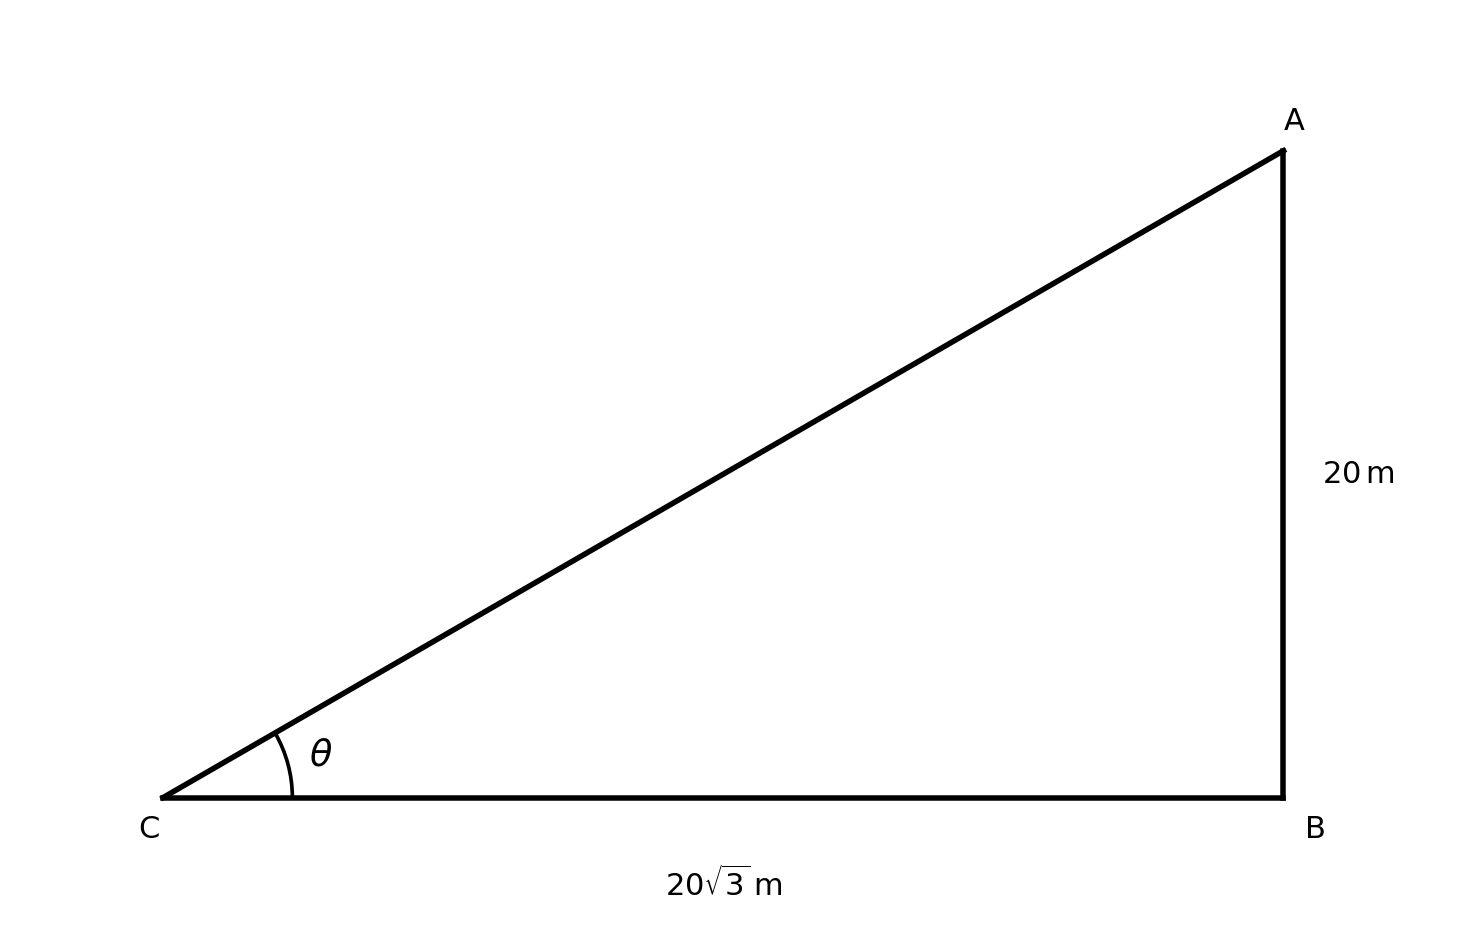
\includegraphics[width=0.83\linewidth]{figs/Tower.png}
    \caption{Tower and shadow; dimensions match the marking scheme.}
    \label{fig:class10-tower}
\end{figure}
\solution
The angle of elevation of the Sun is $\theta$. In right triangle $ABC$,
\begin{align}
 \tan\theta&=\frac{AB}{BC}=\frac{20}{20\sqrt{3}}=\frac{1}{\sqrt{3}},\
 \therefore\quad \boxed{\theta=30^\circ}.
\end{align}
The length $20\sqrt{3}\,\mathrm{m}$ is confirmed by the CBSE 2015 Class X marking scheme. The earlier source transcription omitted the radical and multiplier.

The figure was generated by the following Python script:
\begin{lstlisting}[frame=single,basicstyle=\rmfamily,escapeinside={(*@}{@*)}]
(*@\makebox[\dimexpr\linewidth-2\fboxsep-2\fboxrule\relax][c]{codes/Tower.py}@*)
\end{lstlisting}

\item Two different dice are tossed together. Find the probability that the product of the two numbers on the top of the dice is $6$. \hfill (CBSE Class X, 2015, Q3)

\solution
The two dice produce $6\times6=36$ equally likely ordered outcomes. The favourable ordered pairs are
\begin{align}
 (1,6),\ (6,1),\ (2,3),\ (3,2).
\end{align}
There are four favourable outcomes. Thus,
\begin{align}
 P(\text{product}=6)&=\frac{4}{36}=\boxed{\frac{1}{9}}.
\end{align}

\item In Figure \ref{fig:class10-chord-tangent}, $PQ$ is a chord of a circle with centre $O$ and $PT$ is a tangent. If $\angle QPT=60^\circ$, find $\angle PRQ$. \hfill (CBSE Class X, 2015, Q4)
\begin{figure}[H]
    \centering
    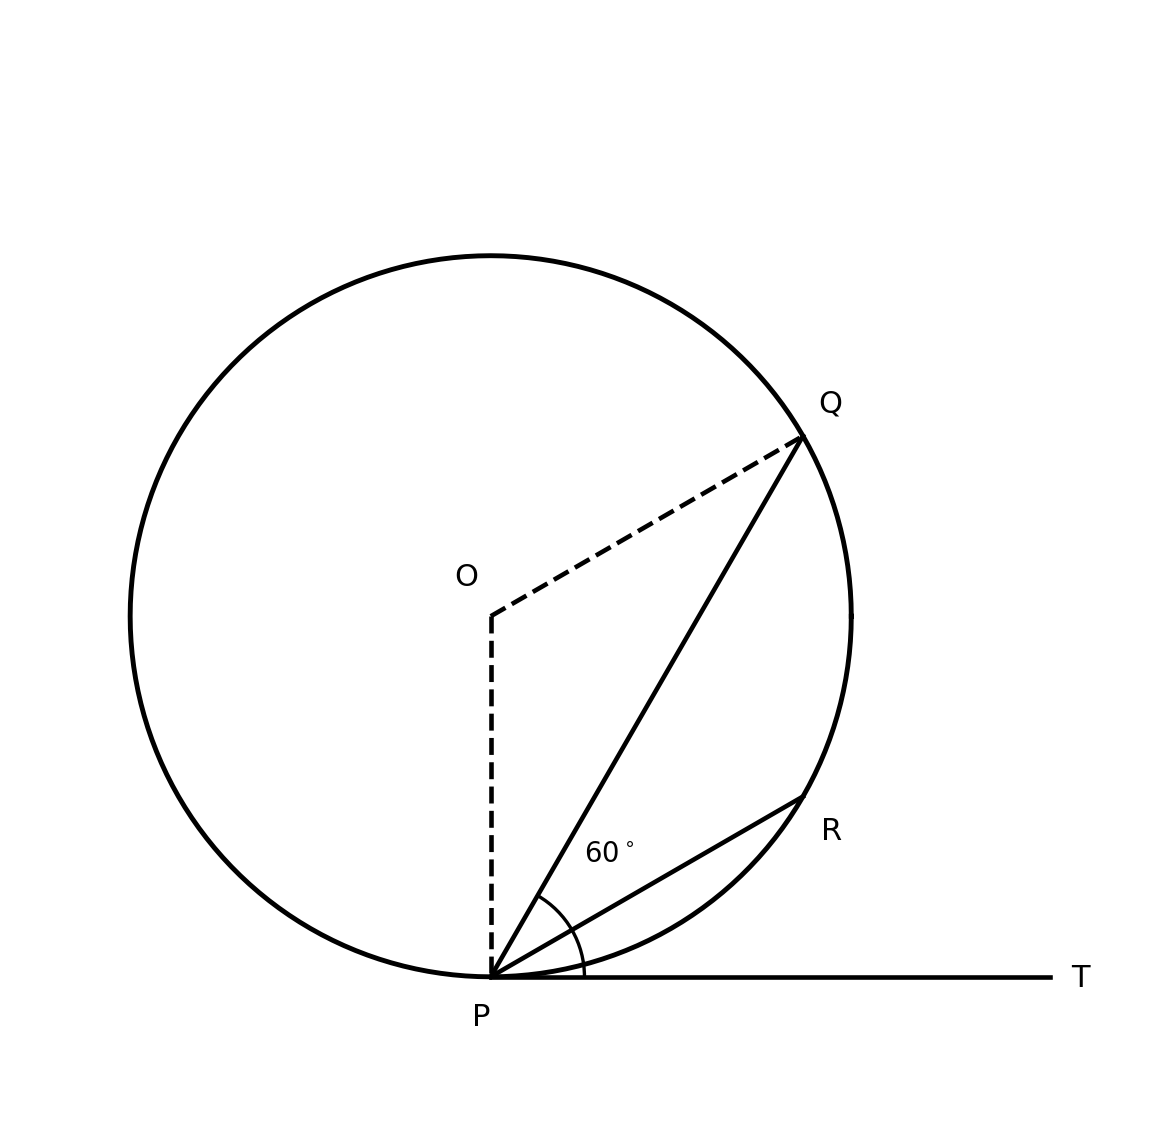
\includegraphics[width=0.66\linewidth]{figs/TangentChord.png}
    \caption{Chord and tangent configuration; drawn by Python.}
    \label{fig:class10-chord-tangent}
\end{figure}
\solution
Since a radius is perpendicular to the tangent at the point of contact, $\angle OPT=90^\circ$. Hence
\begin{align}
 \angle OPQ&=\angle OPT-\angle QPT=90^\circ-60^\circ=30^\circ.
\end{align}
As $OP=OQ$, triangle $OPQ$ is isosceles, so $\angle OQP=30^\circ$ and
\begin{align}
 \angle POQ&=180^\circ-30^\circ-30^\circ=120^\circ.
\end{align}
The point $R$ lies on the minor arc $PQ$ in the given figure. Therefore $\angle PRQ$ subtends the major arc $PQ$, whose measure is $360^\circ-120^\circ=240^\circ$. Thus
\begin{align}
 \angle PRQ&=\frac{240^\circ}{2}=\boxed{120^\circ}.
\end{align}

The figure was generated by the following Python script:
\begin{lstlisting}[frame=single,basicstyle=\rmfamily,escapeinside={(*@}{@*)}]
(*@\makebox[\dimexpr\linewidth-2\fboxsep-2\fboxrule\relax][c]{codes/TangentChord.py}@*)
\end{lstlisting}

\end{enumerate}

\subsection{Section B}
\begin{enumerate}[label=\thesubsection.\arabic*,ref=\thesubsection.\theenumi,start=5]
\numberwithin{equation}{enumi}

\item Two tangents $RQ$ and $RP$ are drawn from an external point $R$ to a circle with centre $O$. If $\angle PRQ=120^\circ$, prove that $OR=PR+RQ$. \hfill (CBSE Class X, 2015, Q5)
\begin{figure}[H]
    \centering
    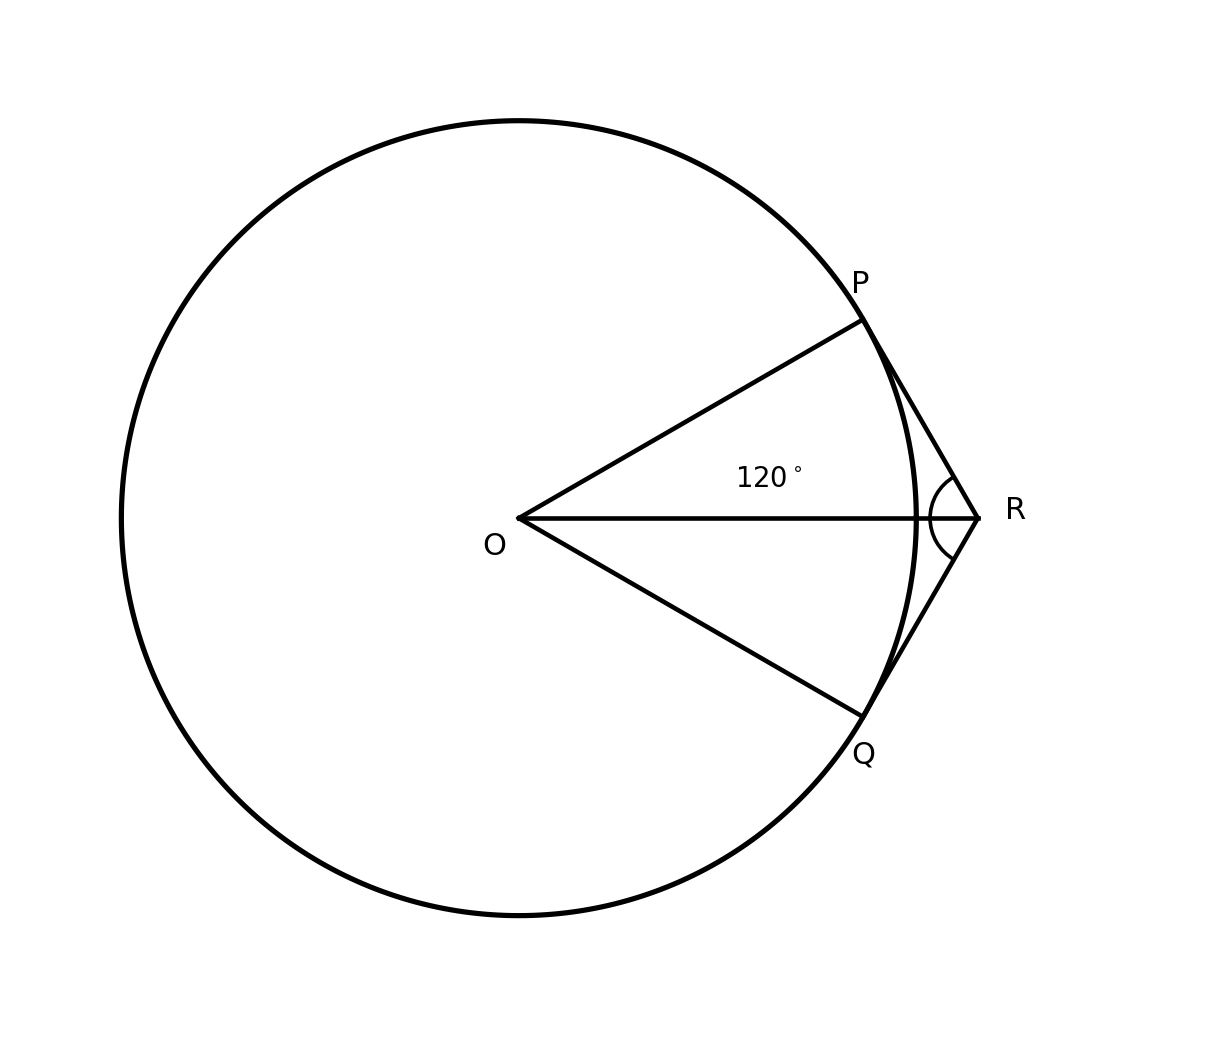
\includegraphics[width=0.64\linewidth]{figs/TwoTangents.png}
    \caption{Two tangents from an external point; drawn by Python.}
    \label{fig:class10-two-tangents}
\end{figure}
\solution
The radii to the points of contact are perpendicular to the tangents: $OP\perp PR$ and $OQ\perp QR$. The right triangles $\triangle OPR$ and $\triangle OQR$ are congruent by RHS, since $OP=OQ$ and $OR$ is common. Hence
\begin{align}
 PR=RQ,\qquad \angle PRO=\frac{1}{2}\angle PRQ=60^\circ.
\end{align}
In right triangle $OPR$,
\begin{align}
 \cos60^\circ&=\frac{PR}{OR}\\
 \frac{1}{2}&=\frac{PR}{OR}\\
 OR&=2PR.
\end{align}
Using $PR=RQ$ gives
\begin{align}
 \boxed{OR=PR+RQ}.
\end{align}

The figure was generated by the following Python script:
\begin{lstlisting}[frame=single,basicstyle=\rmfamily,escapeinside={(*@}{@*)}]
(*@\makebox[\dimexpr\linewidth-2\fboxsep-2\fboxrule\relax][c]{codes/TwoTangents.py}@*)
\end{lstlisting}
\end{enumerate}

\subsection{Batch audit}
Questions 1--5 in this batch are now based on the official 2015 Class X wording and figure configuration. The chapter ordering separates Question 5 into Section B, matching the official paper. Continue auditing the remaining questions against the official paper before submission.


\end{document}
